\documentclass{beamer}

\mode<presentation>
{
  \usetheme{Frankfurt}
  \setbeamercovered{transparent}
  \usecolortheme{wolverine}
}

\usepackage[english]{babel}
\usepackage[latin1]{inputenc}
\usepackage{times}
\usepackage[T1]{fontenc} 
\usepackage{tikz}
% Or whatever. Note that the encoding and the font should match. If T1
% does not look nice, try deleting the line with the fontenc.
\usepackage{amsmath}

\newcommand{\linespace}{\vskip 0.25cm}

\definecolor{MyForestGreen}{rgb}{0,0.7,0} 
\newcommand{\tableemph}[1]{{#1}}
\newcommand{\tablewin}[1]{\tableemph{#1}}
\newcommand{\tablemid}[1]{\tableemph{#1}}
\newcommand{\tablelose}[1]{\tableemph{#1}}

\definecolor{MyLightGray}{rgb}{0.6,0.6,0.6}
\newcommand{\tabletie}[1]{\color{MyLightGray} {#1}}

% The text in square brackets is the short version of your title and will be used in the
% header/footer depending on your theme.
\title[Usability of Error Messages for Introductory Students]{Usability of Error Messages For \\ Introductory Students}

% Sub-titles are optional - uncomment and edit the next line if you want one.
% \subtitle{Why does sub-tree crossover work?} 

% The text in square brackets is the short version of your name(s) and will be used in the
% header/footer depending on your theme.
\author[Schliep]{Paul A. Schliep}

% The text in square brackets is the short version of your institution and will be used in the
% header/footer depending on your theme.
\institute[U of Minn, Morris]
{
  Division of Science and Mathematics \\
  University of Minnesota, Morris \\
}

% The text in square brackets is the short version of the date if you need that.
\date[April '15] % (optional)
{25 April 2015}

% Delete this, if you do not want the table of contents to pop up at
% the beginning of each subsection:
\AtBeginSection[]
{
  \begin{frame}<beamer>
    \frametitle{Outline}
    \tableofcontents[currentsection, hideothersubsections]
  \end{frame}
}

\begin{document}

\begin{frame}
  \titlepage
\end{frame}

% For a 20-25 minute senior seminar talk you probably want something like:
% - Two or three major sections (other than the summary).
% - At *most* three subsections per section.
% - Talk about 30s to 2min per frame. So there should probably be between
%   15 and 30 frames, all told.

\section*{Introduction}

\subsection*{Overview of error messages}

\begin{frame}[fragile]
  \frametitle{Introduction to error messages}
  \begin{itemize}
  	\item Mistakes happen a lot in programming
  	\begin{itemize}
  		\item especially for new programmers
  	\end{itemize}
  	\item Error messages produced from programming mistakes
  	\item Tells the user information about the issue
  	\item Here's an example of an error message (in Java):
  	\begin{itemize}
  		\item \texttt{->} denotes output
  	\end{itemize}
  	  \begin{verbatim}
int three = 3;
System.out.print(tree);

-> error: 
`tree' cannot be resolved to a variable
  	\end{verbatim}
  \end{itemize}
\end{frame}

\begin{frame}
  \frametitle{Importance of error messages}
  \begin{itemize}
    \item Analyze error messages from usability perspective
  	\item Error messages are important tool for beginner programmers
  	\begin{itemize}
  		\item one of the primary interactions between the system and the user
  	\end{itemize}
  	\item A good error message should:
  	\begin{itemize}
  		\item convey the actual issue
  		\item help a student locate the issue
  		\item not add confusion
  	\end{itemize}
  	\item Unhelpful error messages create frustration
  \end{itemize}
\end{frame}

%\begin{frame}[fragile]
%	\frametitle{Example of poor error message}
%	\begin{verbatim}
%	developing...
%	\end{verbatim}
%\end{frame}

%\begin{frame}[fragile]
%  \frametitle{Overview of research and motivation}
%  \begin{itemize}
%  	\item Analyze error messages from usability perspective
%  	\item 
%  \end{itemize}
%\end{frame}

\subsection*{Outline}

\begin{frame}
  \frametitle{Outline}
  \tableofcontents
\end{frame}

\section[Background]{Background}

\subsection{Compiler and runtime errors}

\begin{frame}[fragile]
	\frametitle{Compiler errors}
		\begin{itemize}
			\item Compiler: converts code to lower level language so instructions can be computed
			\item Compiler errors occur when code cannot be compiled due to errors
			\item Program will not execute
			\item For newer programmers, these typically occur from syntax errors
			\item Example (in Java):
			\begin{verbatim}
		int seven = (2 + 5;
		
		-> error: ')' expected
			\end{verbatim}
		\end{itemize}
\end{frame}

\begin{frame}[fragile]
	\frametitle{Runtime errors}
		\begin{itemize}
			\item Runtime error occurs after a program has compiled, during execution of the program
			\item Dependent on values that may not be known at compile time
			\item Usually indication of logical errors in the code
			\item Example:
			\begin{verbatim}
String theString = "hello";
int low = 3;
int high = 6;
System.out.print(theString.substring(low,high));

-> java.lang.StringIndexOutOfBoundsException:
String index out of range: 6
			\end{verbatim}
		\end{itemize}
\end{frame}

\subsection{Dynamic and statically typed}

\begin{frame}[fragile]
  \frametitle{Statically typed languages}
	\begin{itemize}
		\item Variables assigned types
		\item Type checking done at compile time
		\item Following code would give compile time error
		\begin{verbatim}
		String personName = "Frank";
		personName = 7;
		\end{verbatim}
	\end{itemize}
\end{frame}

\begin{frame}[fragile]
  \frametitle{Dynamically typed languages}
	\begin{itemize}
		\item Variables are not assigned to types
		\item Type checking done at runtime
		\item Following would give runtime error
		\begin{verbatim}
		var x = "Frank";
		var y = 7;
		x - y;
		\end{verbatim}
	\end{itemize}
\end{frame}

\section[Analyses]{Analyses of error messages}

\subsection[DrRacket Analysis]{Analysis of Racket and DrRacket}

\begin{frame}[fragile]
	\frametitle{Racket programming language}
		\begin{itemize}
			\item Racket: Programming language useful for teaching in introductory courses
			\item Functional language: computation as a composition of functions, retains immutable data, avoids changing state
			\item Dynamically typed
			\item Syntax example:
			\begin{verbatim}
			(+ 1 2)

			-> 3
			\end{verbatim}
		\end{itemize}

\end{frame}

\begin{frame}
	\frametitle{DrRacket integrated development environment}
		\begin{itemize}
			\item An integrated development environment (IDE) is a program for writing and running code along with debugging tools
			\item DrRacket is an IDE for developing programs in Racket
			\item Geared toward introductory programmers
			\item DrRacket offers user-friendly error messages and libraries
		\end{itemize}
		
\end{frame}

%\begin{frame}
%	\frametitle{DrRacket interface}
%%			\includegraphics[keepaspectratio, width= 1.0 \textwidth]%{drracketGUI.png}

%\end{frame}

\begin{frame}
	\frametitle{Study of DrRacket error messages}
		\begin{itemize}
		  	\item Marceau et al. noticed students struggling with error messages in course
		  	\item Interested in which errors students struggled with
			\item Conducted study on DrRacket error messages in Spring 2010
			\item Hoping to use data to improve student interactions with DrRacket error messages

		\end{itemize}
\end{frame}
		
\begin{frame}
	\frametitle{Method}
 		\begin{itemize}
			\item Configured DrRacket to save a copy of each program from 6 consecutive lab sessions
			\item Measured errors students responded poorly to
			\item Group errors into nine related categories
 		\end{itemize}
\end{frame}

\begin{frame}
	\frametitle{Table of results}
	\begin{tikzpicture}[remember picture,overlay]
            \node[at=(current page.center)] {
                \includegraphics[width=\paperwidth]{MEE-data.pdf}
            };
        \end{tikzpicture}
	%\includegraphics[width=\paperwidth]{MEE-data.pdf}

\end{frame}

%\begin{frame}[fragile]
% \frametitle{Student code example}
%				\textcolor{orange}{
%				\texttt{
%;; Locates bias or name from 2 words
%}}

% 			\begin{verbatim}
%1 (define (label-near? name bias word1 word2)
%2   (cond
%3      (and (cond [(string=? name word1) 
%4                    "Name Located"]
%5                 [(string=? bias word2)
%6                    "Bias Located"])
%7           (cond [(string=? name word2)
%8                    "Name Located"]
%9                 [(string=? bias word2) 
%10                   "Bias Located"])
%11    "Mark")))
%-> and: found a use of `and' that does not follow 
%an open parenthesis
%\end{verbatim}
%\end{frame}

\begin{frame}
 \frametitle{Student edit example}
 \begin{itemize}
 \item Missing parentheses before \texttt{cond} on line 2
 \item Same error message produced for each edit
 \end{itemize}
 	%\begin{tikzpicture}[remember picture,overlay]
      %      \node[at=(current page.center)] {
      %          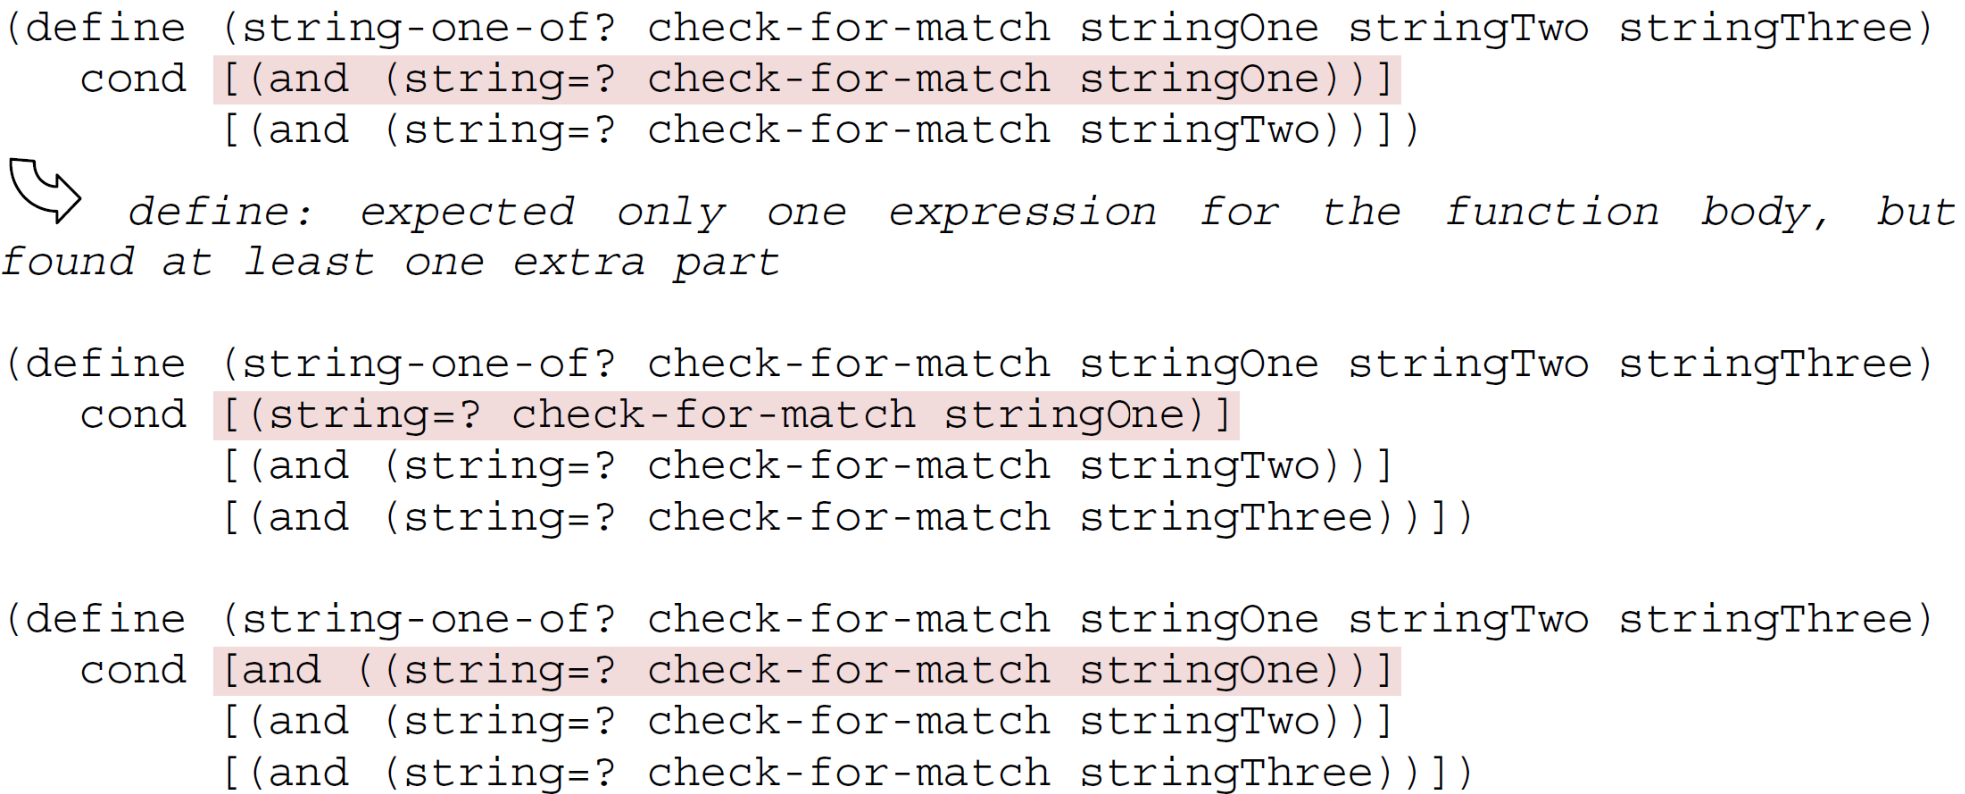
\includegraphics[width=\paperwidth]{RacketStudentEditPt1.pdf}
      %      };
      %  \end{tikzpicture}
      \
      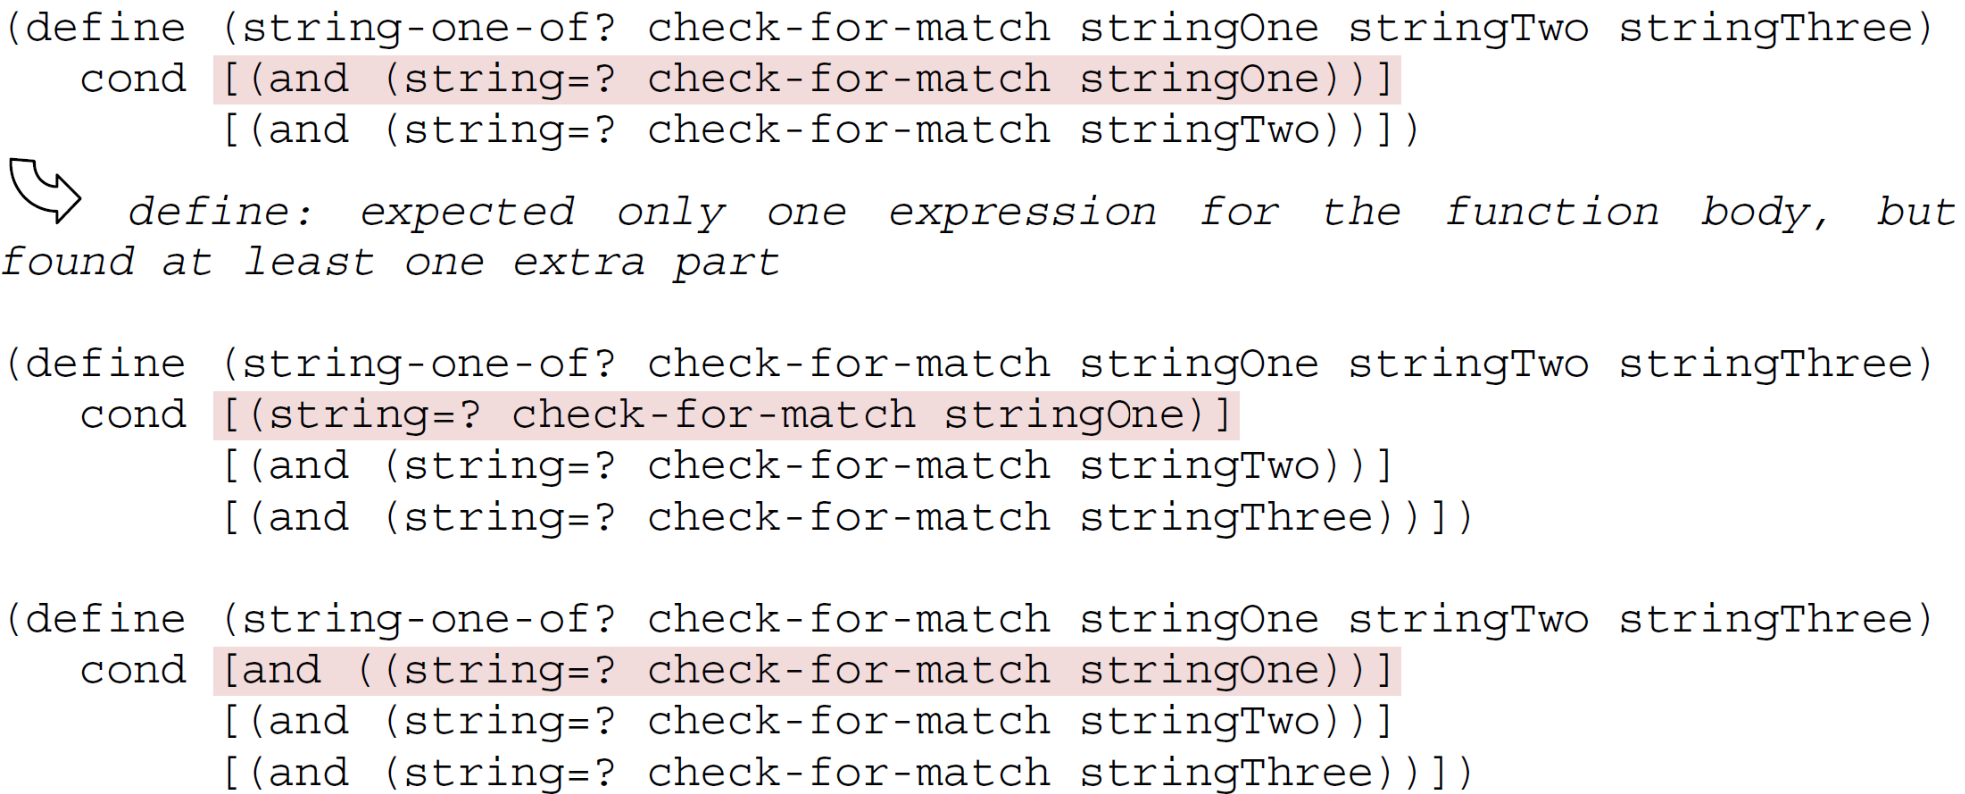
\includegraphics[width=0.9\paperwidth]{RacketStudentEditPt1.pdf}
      		\\
		\only{\tiny{Marceau et al.}}
\end{frame}

\begin{frame}[fragile]
 \frametitle{Student edit example continued}
 	%\begin{tikzpicture}[remember picture,overlay]
       %     \node[at=(current page.center)] {
       %         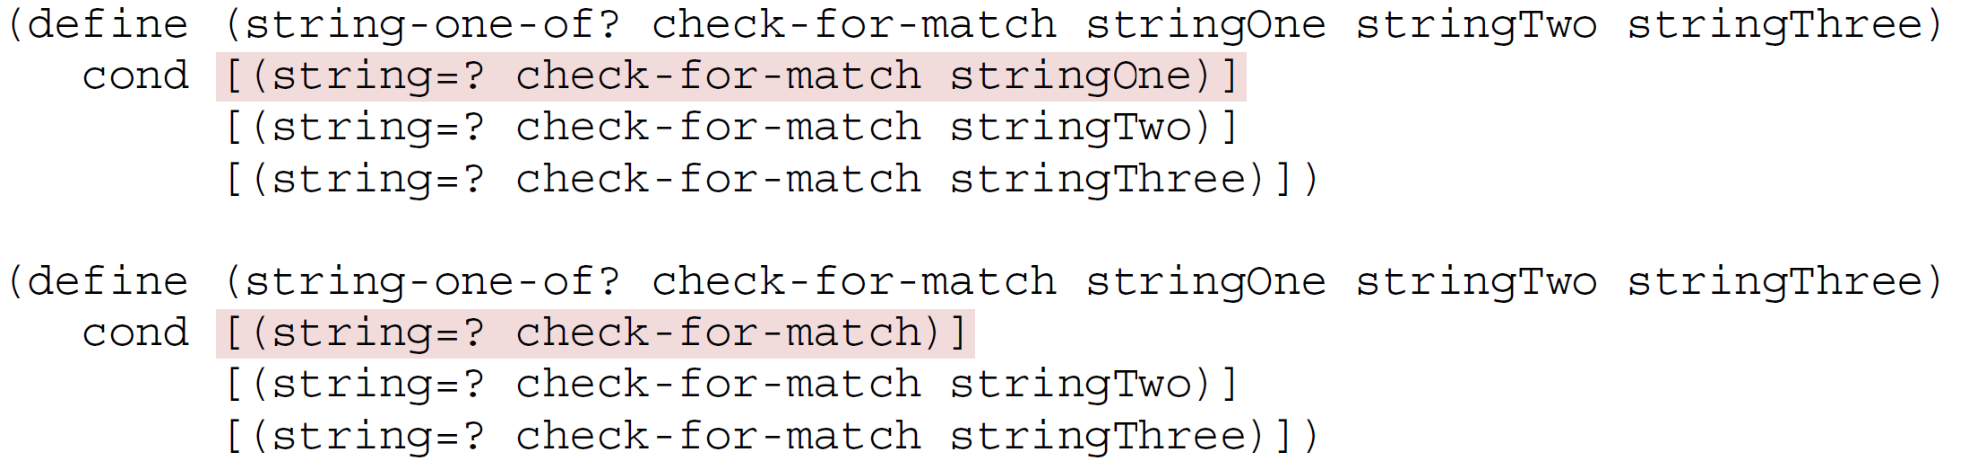
\includegraphics[width=\paperwidth]{RacketStudentEditPt2.pdf}
       %     };
       % \end{tikzpicture}
       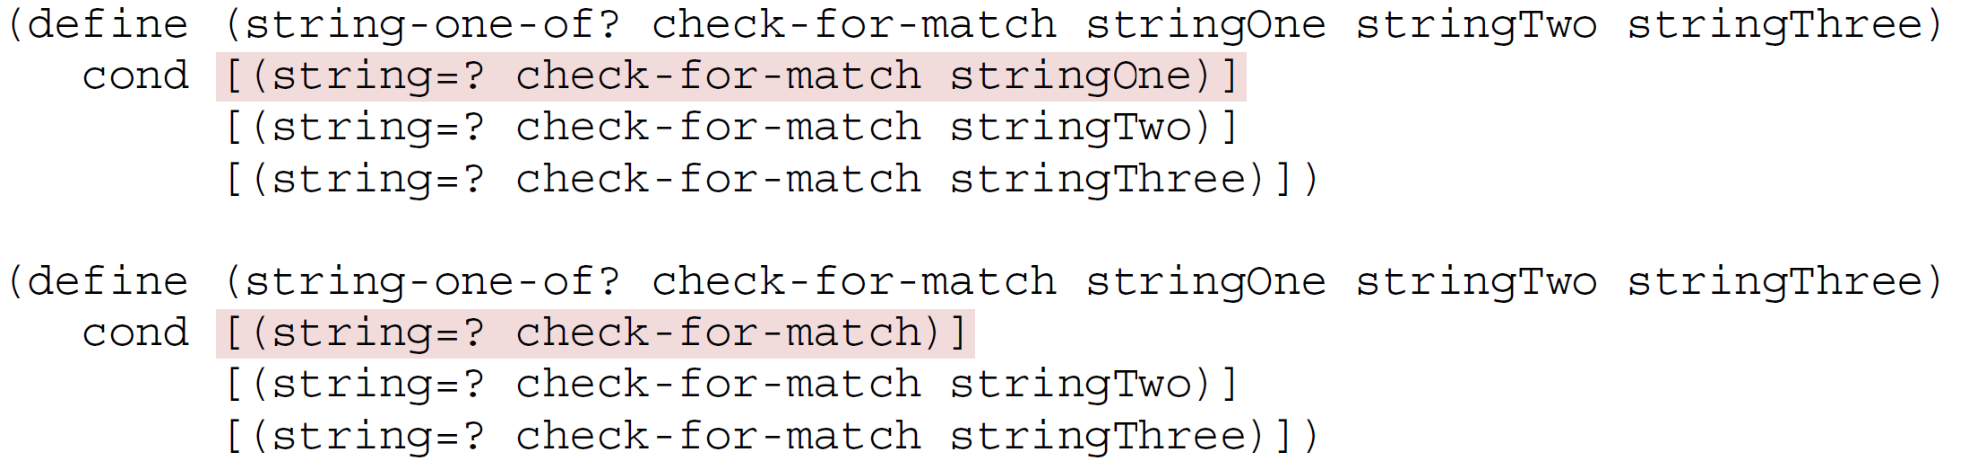
\includegraphics[width=0.9\paperwidth]{RacketStudentEditPt2.pdf}
       		\\
		\only{{\tiny Marceau et al.}}
		
		\begin{itemize}
 			\item Student did not fix error
 			\item Fixed code:
		\end{itemize}
		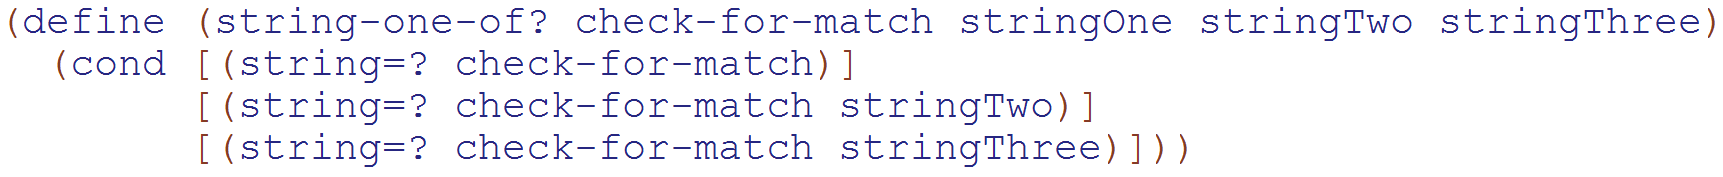
\includegraphics[width=0.9\paperwidth]{fixedCode.png}
%		\scriptsize{
%		\begin{verbatim}
%(define (string-one-of? check-for-match stringOne stringTwo stringThree)
%  (cond [(string=? check-for-match)]
%        [(string=? check-for-match stringTwo)]
%        [(string=? check-for-match stringThree)]))
%		\end{verbatim}}
\end{frame}

\begin{frame}
	\frametitle{Results}
		\begin{itemize}
			\item Errors that were difficult to resolve was relative to course material
			\item Some errors were not indicator of underlying issue
			\begin{itemize}
				\item students struggled with these errors
				\item suggests issues in error message effectiveness
			\end{itemize}
			\item Further research on understanding actual underlying errors and improving DrRacket error messages
		\end{itemize}
\end{frame}

\subsection[Compiler Analysis]{Analysis of compiler errors}

\begin{frame}
	\frametitle{Analysis of compiler errors}
		\begin{itemize}
			\item Students struggle with compiler error messages in course taught by V. Javier Traver at Jaume I University
			\item Traver interested in finding compiler error messages students struggled with
			\item Conducted study in Fall 2010
				\begin{itemize}
				\item course used C++ programming language
				\end{itemize}
			\item Study from a strictly usability perspective
			\begin{itemize}
				\item did not consider technical constraints
			\end{itemize}
		\end{itemize}

\end{frame}

\begin{frame}[fragile]
	\frametitle{Intro to C++}
		\begin{itemize}
			\item C++: Programming language not designed to be taught in intro course
			\item Imperative language: uses memory manipulation and state-changing statements
			\item Statically-typed
			\item Syntax example:
			\begin{verbatim}
			int a = 2;
			a = a + 2;
			cout << a << endl;
			
			-> 4
			\end{verbatim}
		\end{itemize}

\end{frame}

\begin{frame}
	\frametitle{Method of study}
		\begin{itemize}
			\item GNU g++ compiler used
			\item Erroneous student code gathered from semester
			\item Analyzed each message:
			\begin{itemize}
				\item why the error occurred
				\item possible alternative error message
				\item why the error message is unhelpful
			\end{itemize}
		\end{itemize}

\end{frame}

\begin{frame}[fragile]
	\frametitle{Example of code analyzed}
Offending code (missing curly brace):
\begin{verbatim}
1 SavingAccount::SavingAccount(){
2     float SavingAccount::getInterestRate(){
3    	  return rate;
4     }
\end{verbatim}

Error message:
\begin{verbatim}
In method 'SavingAccount::SavingAccount()':
declaration of 
'float SavingAccount::getInterestRate()'
outside of class is not definition
\end{verbatim}

\end{frame}

\begin{frame}[fragile]
	\frametitle{Example continued}
Alternative error message:
\begin{verbatim}
A function declaration inside a function body is 
not possible. Did you forget '}' to close the 
body of the previous function definition?
\end{verbatim}

\begin{itemize}
	\item Original error is confusing
	\begin{itemize}
		\item does not tell user missing curly brace
	\end{itemize}
\end{itemize}

\end{frame}

\begin{frame}
	\frametitle{Results}
		\begin{itemize}
			\item No quantitative data, just observations
			\item Hopes that approaches be considered to improve messages
			\item Future work: develop methods to improve messages in course
		\end{itemize}

\end{frame}

\section[Methodologies]{Methodologies for improving error messages}

\subsection[DrRacket recommendations]{Recommendations for improving IDE error messages}

\begin{frame}
	\frametitle{Recommendations}
		\begin{itemize}
			\item Recommendations on error message design
			\item Marceau et al. used previous research
			\item Wanted to maintain two design principles:
			\begin{itemize}
				\item error messages should not propose solutions
				\item error messages should not prompt toward incorrect edits
			\end{itemize}
		\end{itemize}

\end{frame}

\begin{frame}[fragile]
	\frametitle{Recommendations continued}
		\begin{itemize}
			\item Simplify message vocabulary
				\begin{itemize}
					\item eg, student will understand \texttt{variable} more than \texttt{identifier}
					\item these should be for lower levels in DrRacket
				\end{itemize}
			\item Be explicit with highlighting
			\item Color coding references with its corresponding code
		\end{itemize}

\end{frame}

\begin{frame}
	\frametitle{Poor highlighting example}
	\begin{itemize}
		\item Runtime error, never refers to highlighted expression
	\end{itemize}
		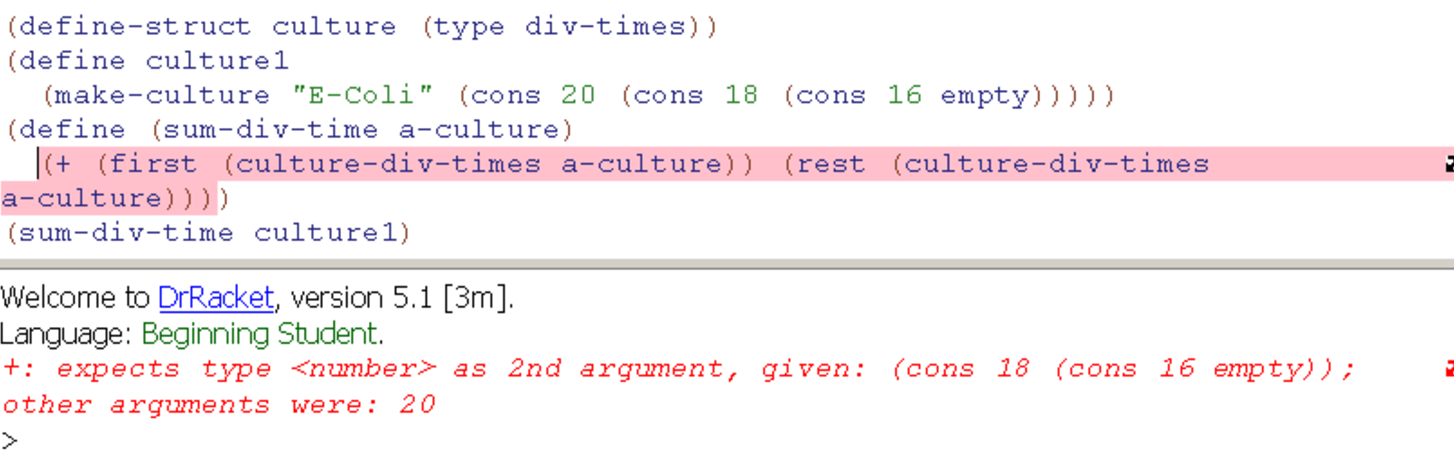
\includegraphics[keepaspectratio, width=0.95\paperwidth]{DrRacketNoClearReferent.pdf}
		\\
		\only{\tiny{Marceau et al.}}
\end{frame}

\begin{frame}
	\frametitle{Color coded error message}
	Red highlights definition, green highlights clause, blue highlights definition \\~\\
		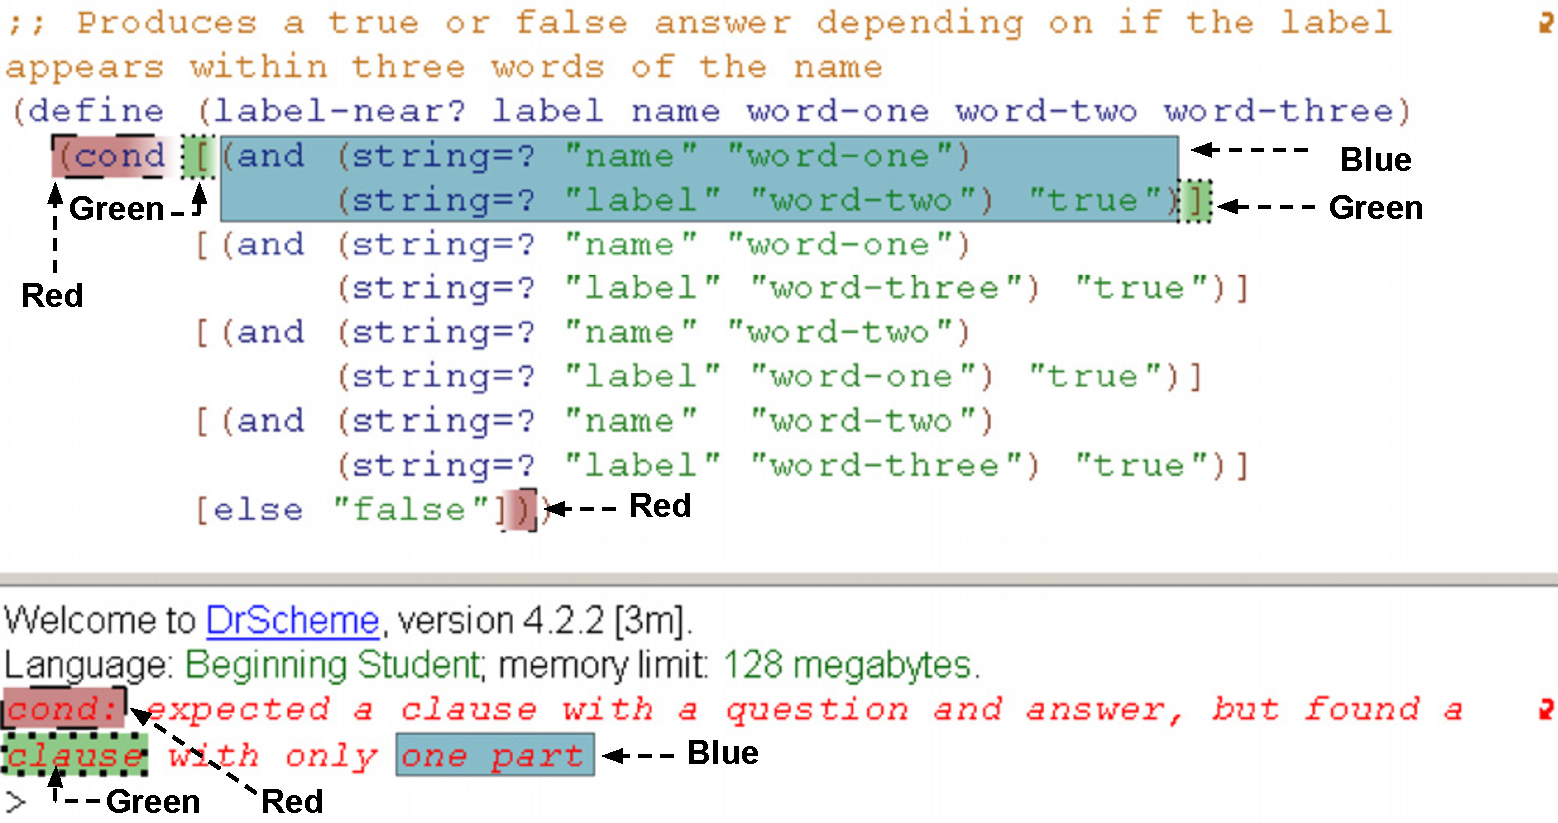
\includegraphics[keepaspectratio, width=0.85\paperwidth]{ColorCodedMessage.pdf}
		\\
		\only{\tiny{Marceau et al.}}
\end{frame}

\begin{frame}
	\frametitle{Future work}
		\begin{itemize}
			\item How to Design Programs (HtDP) libraries for DrRacket
			\item Further research needed to evaluate HtDP libraries
		\end{itemize}

\end{frame}

\subsection[Syntax error enhancement]{Analysis of syntax error enhancement}

\begin{frame}
	\frametitle{Intro to syntax errors}
		\begin{itemize}
			\item Syntax errors when learning a new language
			\item "Syntax errors can be a significant barrier to student success"  - Denny et al.
			\item Denny et al. propose to improve syntax error messages
		\end{itemize}

\end{frame}

\begin{frame}
	\frametitle{Improving errors}
		\begin{itemize}
			\item Course used Java, language similar to C++
			\item Course also used CodeWrite, online IDE
			\item Pulled student submissions from CodeWrite
			\item Match common erroneous code, extracted line containing error, and inserted their enhanced error
		\end{itemize}

\end{frame}

\begin{frame}[fragile]
	\frametitle{Syntax error}
	Erroneous code:
	\begin{verbatim}
	if (score < 0) || (score > 100)
	
	-> Syntax error on token "||", if expected
	\end{verbatim}
\end{frame}

\begin{frame}
	\frametitle{Enhanced syntax error example}
		\begin{tikzpicture}[remember picture,overlay]
            \node[at=(current page.center)] {
                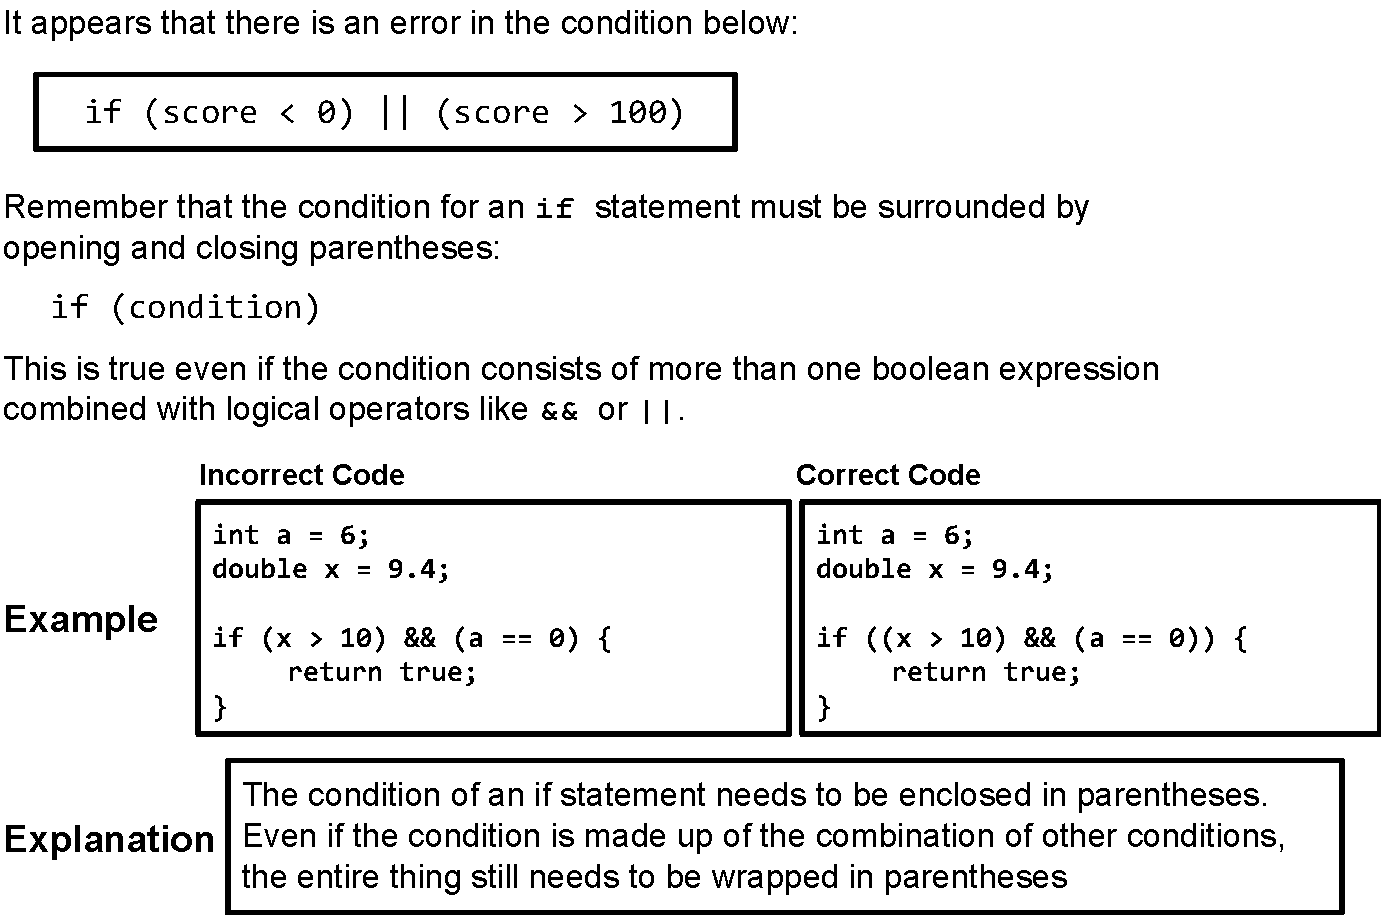
\includegraphics[width=0.80\paperwidth]{EnhancedSyntaxErrorSlide.pdf}
            };
        \end{tikzpicture}
              		\\
		\only{\tiny{Denny et al.}}
	%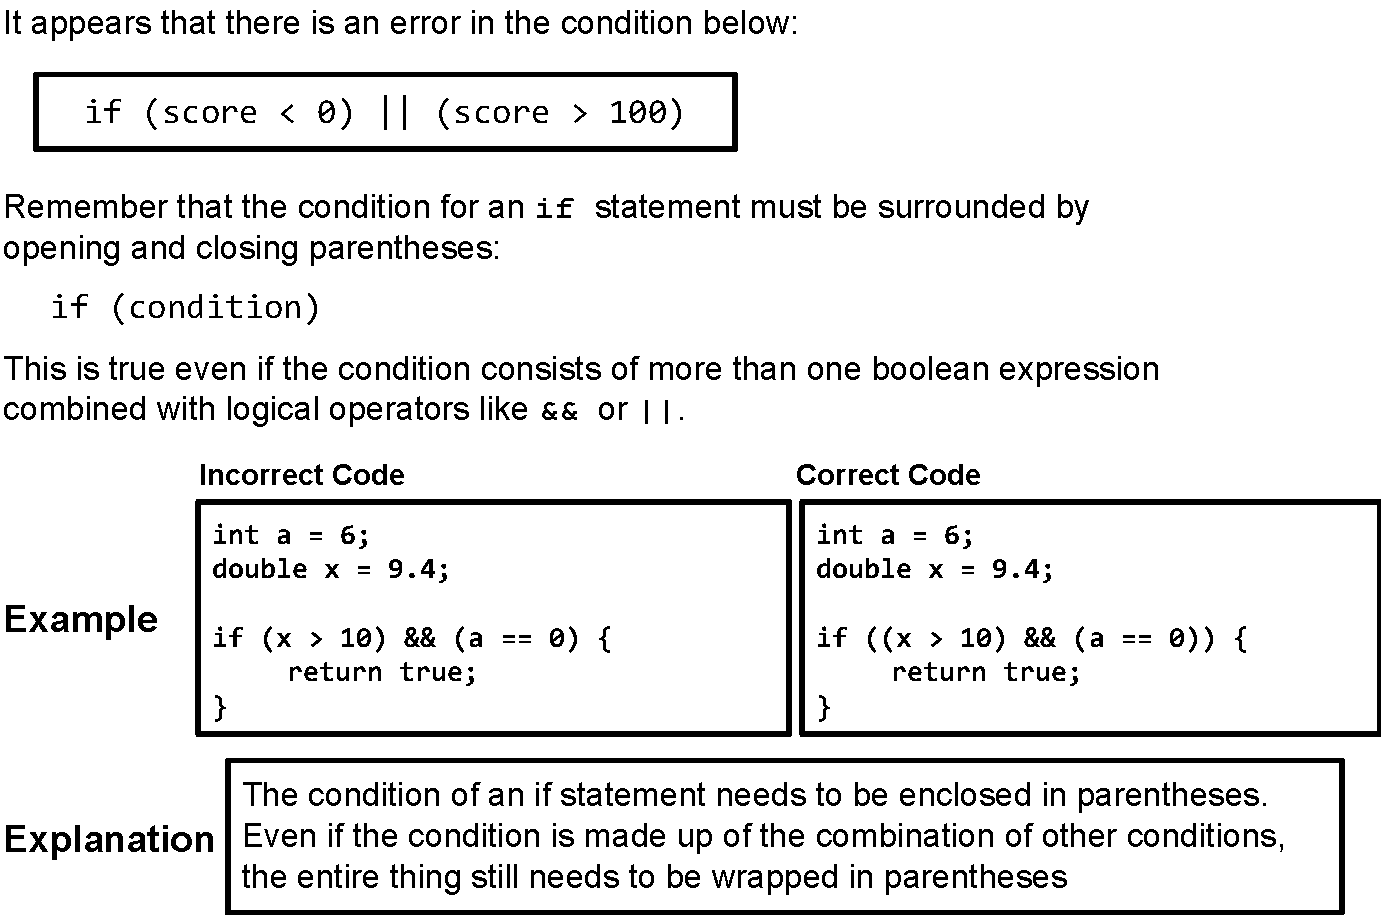
\includegraphics[keepaspectratio, width=0.8 \textwidth]{EnhancedSyntaxErrorSlide.pdf}
\end{frame}

\begin{frame}
	\frametitle{Testing the enhanced syntax messages}
		\begin{itemize}
			\item Students from course in control group (original error messages) and intervention group (enhanced error messages)
			\item Compared attempts of student submissions
			\item Used t-tests to find results
			\begin{itemize}
				\item t-test: finds if there is statistically significant difference between two data groups
			\end{itemize}
		\end{itemize}

\end{frame}

\begin{frame}
	\frametitle{Results of syntax enhancement}
		\begin{itemize}
			\item t-tests gave high p-values (p > 0.05)
				\begin{itemize}
				\item indication of no evidence of statistically significant difference
				\item note: not all tests shown
				\item this test compares longest consecutive failing submissions 
				\end{itemize}
			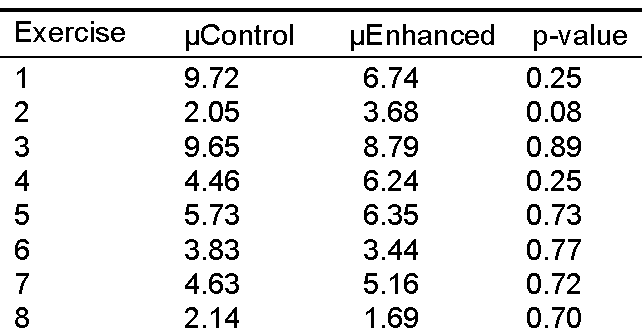
\includegraphics[keepaspectratio, width=0.75\textwidth]{EnhancedSyntaxData.pdf}
		\end{itemize}

\end{frame}

\begin{frame}
	\frametitle{Future work}
		\begin{itemize}
			\item Denny et al. believed several factors were the cause for no significance
			\begin{itemize}
				\item may not have paid attention to additional information
				\item examples not relevant to student code
			\end{itemize}
			\item Hope to apply additional research into their messages
		\end{itemize}

\end{frame}


\section[Conclusions]{Conclusions}

\begin{frame}
	\frametitle{Conclusions}
		\begin{itemize}
			\item Error message usability is crucial in programming
			\item More efforts needed on error message usability
			\item Research shows error messages are difficult to deal with
			\begin{itemize}
				\item Marceau et al. found error messages do not always show underlying issue
				\item Study by Traver, compiler error messages show poor usability
				\item Marceau et al. recommendations in HtDP
				\item Denny et al. enhanced syntax error messages were ineffective
			\end{itemize}
		\end{itemize}

\end{frame}

%\begin{frame}
% \frametitle{Conclusions of methodologies}
% 	\begin{itemize}		 			 
%	 \end{itemize}
%\end{frame}

%\begin{frame}
%	\frametitle{Future work}
%		\begin{itemize}
%			\item HtDP libraries implemented Marceau et al. research
%			\item Some work being done to attempt to improve compiler error messages
%			\item Growing interest in computer science
%			\begin{itemize}
%				\item more user-friendly error messages are a necessity
%			\end{itemize}
%		\end{itemize}

%\end{frame}

\begin{frame}
	\frametitle{Acknowledgments}
	I would like to thank the following people:
		\begin{itemize}
			\item My advisor, Elena Machkasova, for helping with my senior seminar and useful feedback on my paper and presentation
			\item Stephen Adams and Jim Hall for providing useful feedback on my paper
			\item Friends and family for attending
	%		\item Paul Schliep, as none of this would have been possible without him
		\end{itemize}

\end{frame}

\section*{References}

\begin{frame} 
	\frametitle{References} 
	
	\begin{thebibliography}{lskdjf}
	
	\bibitem{citeulike:3452411}
Marceau, G., Fisler, K., and Krishnamurthi s.
\newblock Measuring the effectiveness of error messages designed for novice programmers. 2011.

	\bibitem{citeulike:3452411}
Marceau, G., Fisler, K., and Krishnamurthi s.
\newblock Mind your language: On novices' interactions with error messages. 2011.

\bibitem{citeulike:3452411}
Denny, P., Luxton-Reilly, A., and Carpenter, D.
\newblock Enhancing syntax error messages appears ineffectual. 2014.
	
	\bibitem{citeulike:3452411}
	Traver, V.J.
\newblock On compiler error messages: What they say and what they mean. 2010.
  
  	\end{thebibliography}
	
	\linespace
	\begin{center}
	See my seminar paper in "Proceedings of the Thirty-Fourth Computer Science Discipline" for additional references.
	\end{center}
\end{frame} 

\begin{frame}
	\frametitle{Thanks!}
	
	Thank you for your time and I hope you enjoyed the talk
		
	\linespace
	\linespace
	
	Contact:  
	\begin{itemize}
		\item \texttt{schli202@morris.umn.edu}
		\item \url{github.com/Paul-Schliep}
	\end{itemize}
	
	\linespace
	\linespace
	
	\begin{center}
	{\huge Questions?}
	\end{center}
\end{frame}


\end{document}


